
\mojesekce{Open source GIS-based implementation}

\justifying
{\rmfamily The SMODERP2D model belongs to a family of so called
GIS-based hydrological models utilizing capabilities of GIS software
for geodata preprocessing. This part is performed by so-called {\em
GIS providers}. Currently there are two GIS providers implemented.

\begin{itemize}
\item originally only proprietary Esri ArcGIS platform (\url{http://desktop.arcgis.com}) supported
\item new generation comes with a provider suited for open source GRASS GIS platform 
\end{itemize}
}

\subsection{GRASS GIS}
\begin{block}{GRASS GIS}
\begin{columns}
    \begin{column}{0.5\textwidth}
    \centering
    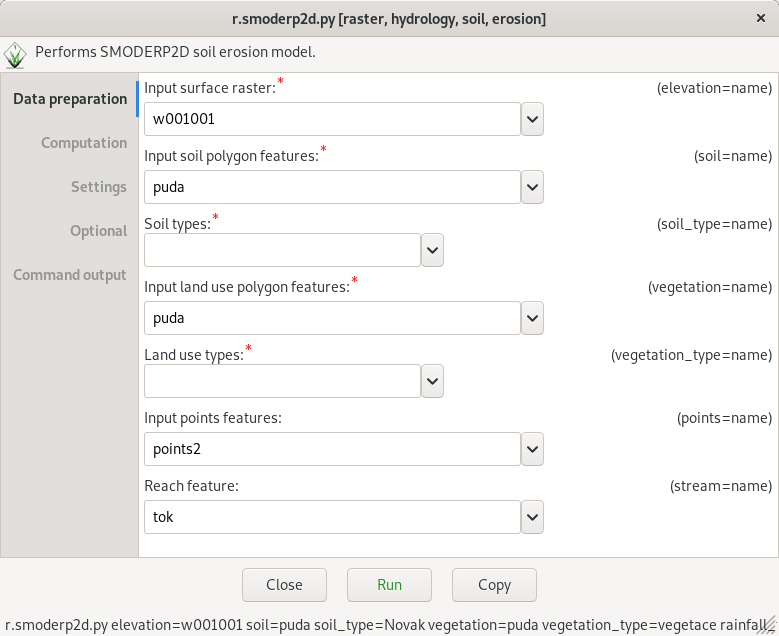
\includegraphics[width = .9\textwidth]{obr/grass.png}
    \end{column}
    \begin{column}{0.5\textwidth}
    
\includegraphics[width = .07\textwidth]{obr/grass-logo.png}
    \justifying
    {\rmfamily {\small
    {\em GRASS} (Geographic Resources Analysis Support System) {\em
    GIS} is a free and open source GIS software suite used for
    geospatial data management and analysis, image processing, spatial
    modeling, and visualization. \newline (\url{http://grass.osgeo.org})}

    \vskip 0.5em

    \begin{itemize}

    \item GRASS-based GIS provider for data preprocessing integrated
    into SMODERP2D codebase
    
    \item {\tt r.smoderp2d} GRASS Addons module for performing
    model computation including data preprocessing

    \end{itemize}
    }
    \end{column}
\end{columns}
\end{block}
\subsection{QGIS}
\begin{block}{QGIS}
\begin{columns}
    \begin{column}{0.5\textwidth}
    
\includegraphics[width = .07\textwidth]{obr/qgis-logo.png}    
    \justifying
    {\rmfamily {\small
    QGIS is a widely known free and open source cross-platform desktop
    geographic information system (GIS) application.}

    \vskip 0.5em

    \begin{itemize}
    
    \item A new QGIS plugin brings the model into QGIS environment
    while data preprocessing part is performed by integrated
    GRASS-based GIS provider
    
    \item QGIS plugin significantly increases accessibility of the
    SMODERP2D model for research purposes and also for engineering
    practice

    \end{itemize}
    
    }

    \end{column}
    \begin{column}{0.5\textwidth}
    \centering
    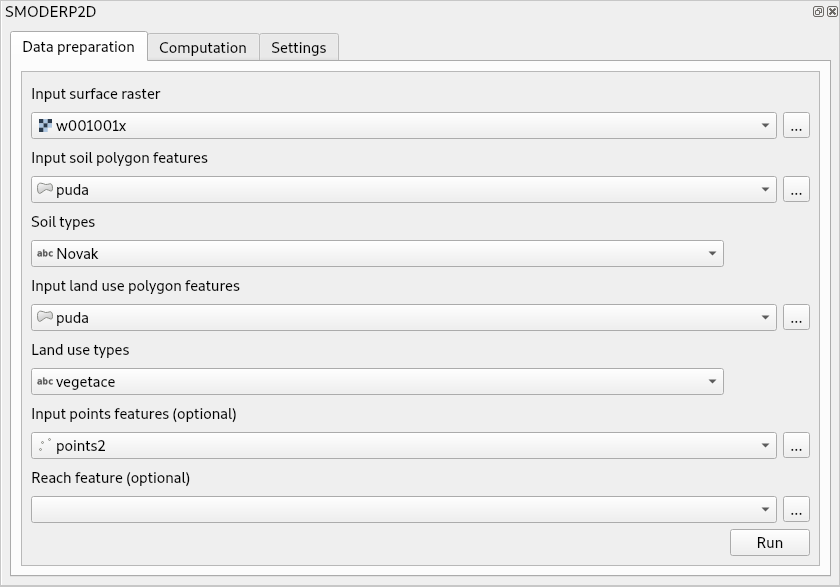
\includegraphics[width = .9\textwidth]{obr/qgis.png}
    \end{column}
\end{columns}
\end{block}

\mojesekce{Conclusions \& Results}
%  \begin{wrapfigure}[8]{r}{0.55\textwidth}
\begin{columns}
    \begin{column}{0.5\textwidth}
        \justifying
        {\rmfamily
        \begin{itemize}
            \item Model is not sensitive to parameter X
            \item Newly derived par. b is lower compared with previous inference
            \item Value of parameter Y corresponds to the previous inference
            \item Soil fractions and textural classes explain only a small portion of parameter values
            \item New generation of SMODERP2D model comes with Esri and GRASS-based GIS providers
        \end{itemize}

        }
    \end{column}
    \begin{column}{0.5\textwidth}
        \justifying
        {\rmfamily
        \begin{itemize}
            \item Accessible via ArcToolbox, GRASS Addons or QGIS plugin
        \end{itemize}
        }
    powered by
    {\tiny
    \begin{lstlisting}
       @ @ @   @       @     @ @     @ @ @     @ @ @ @  @ @ @    @ @ @
      @        @ @   @ @   @     @   @     @   @        @     @  @     @
      @        @   @   @  @       @  @      @  @        @     @  @     @
        @ @    @       @  @       @  @      @  @ @ @    @ @ @    @ @ @
            @  @       @  @       @  @      @  @        @   @    @
            @  @       @   @     @   @     @   @        @    @   @
       @ @ @   @       @     @ @     @ @ @     @ @ @ @  @     @  @

      \  \  /   / /    \   \  /   \  /    /     /        @ @ @   @ @ @
       \ _\/   /_/      \   \/     \/    /_____/        @     @  @     @
           \__/          \  /      _\___/                     @  @      @
               \____      \/      /                          @   @      @
                    \_____/______/                         @     @      @
                                 \                       @       @     @
                                  \____________________ @ @ @ @  @ @ @
    \end{lstlisting}
    }

    \end{column}
\end{columns}


\mojesekce{References}
\justifying
% \small{
{\rmfamily
% \small{
\bibliography{lit}\vspace{0.4cm}
SMODERP2D source code is licensed under GNU
GPL (\url{https://github.com/storm-fsv-cvut/smoderp2d})
% }
}

\mojesekce{Acknowledgment}
\begin{columns}
    \begin{column}{0.4\textwidth}
        \justifying
        {\rmfamily
        The research has been supported by the research grants
        TJ01000270,
        QK1910029,
        and internal CTU grant SGS17/173/OHK1.
        }
    \end{column}
    \begin{column}{0.6\textwidth}
        \centering
        
\includegraphics[height = 5cm]{obr/logo_TACR_dopln_AJ.png}
        
\includegraphics[height = 5cm]{obr/LogoMZeAJ.jpg}
    \end{column}
\end{columns}




% %     \begin{column}{0.4\textwidth}
%     powered by
%     {\tiny
%     \begin{lstlisting}
%        @ @ @   @       @     @ @     @ @ @     @ @ @ @  @ @ @    @ @ @
%       @        @ @   @ @   @     @   @     @   @        @     @  @     @
%       @        @   @   @  @       @  @      @  @        @     @  @     @
%         @ @    @       @  @       @  @      @  @ @ @    @ @ @    @ @ @
%             @  @       @  @       @  @      @  @        @   @    @
%             @  @       @   @     @   @     @   @        @    @   @
%        @ @ @   @       @     @ @     @ @ @     @ @ @ @  @     @  @
% 
%       \  \  /   / /    \   \  /   \  /    /     /        @ @ @   @ @ @
%        \ _\/   /_/      \   \/     \/    /_____/        @     @  @     @
%            \__/          \  /      _\___/                     @  @      @
%                \____      \/      /                          @   @      @
%                     \_____/______/                         @     @      @
%                                  \                       @       @     @
%                                   \____________________ @ @ @ @  @ @ @
%     \end{lstlisting}
%     }
%     \end{column}
% \end{columns}



